
\begin{document}

\maketitle

\section{Introduction}
\begin{frame}[fragile]
  \frametitle{Today}
\begin{itemize}
	\item This introduction
	\begin{itemize}
		\item Getting to know each other
		\item How to get a grade
		\item House rules
		\item Structure of the course
	\end{itemize}
	\item Relationship between business and IT strategy
	\item Architecture
\end{itemize}
	
\end{frame}

\begin{frame}[fragile]
	\frametitle{Andres Kütt}
	\begin{columns}
		\begin{column}[T]{7.5cm}
			\begin{itemize}
				\item Building software for money since 1993
				\item An architect of some capacity for the past 15 years
				\item $\approx$MSc (UT, Statistics), MBA (EBS), MSc (MIT)
				\item Currently chief architect of Estonian information system
				\item Done Skype, a few banks, Estonian Tax and Customs etc. 
				\item Variety of courses and seminars in various schools in Estonia and abroad
			\end{itemize}
		\end{column}
		\begin{column}[T]{2.5cm}
			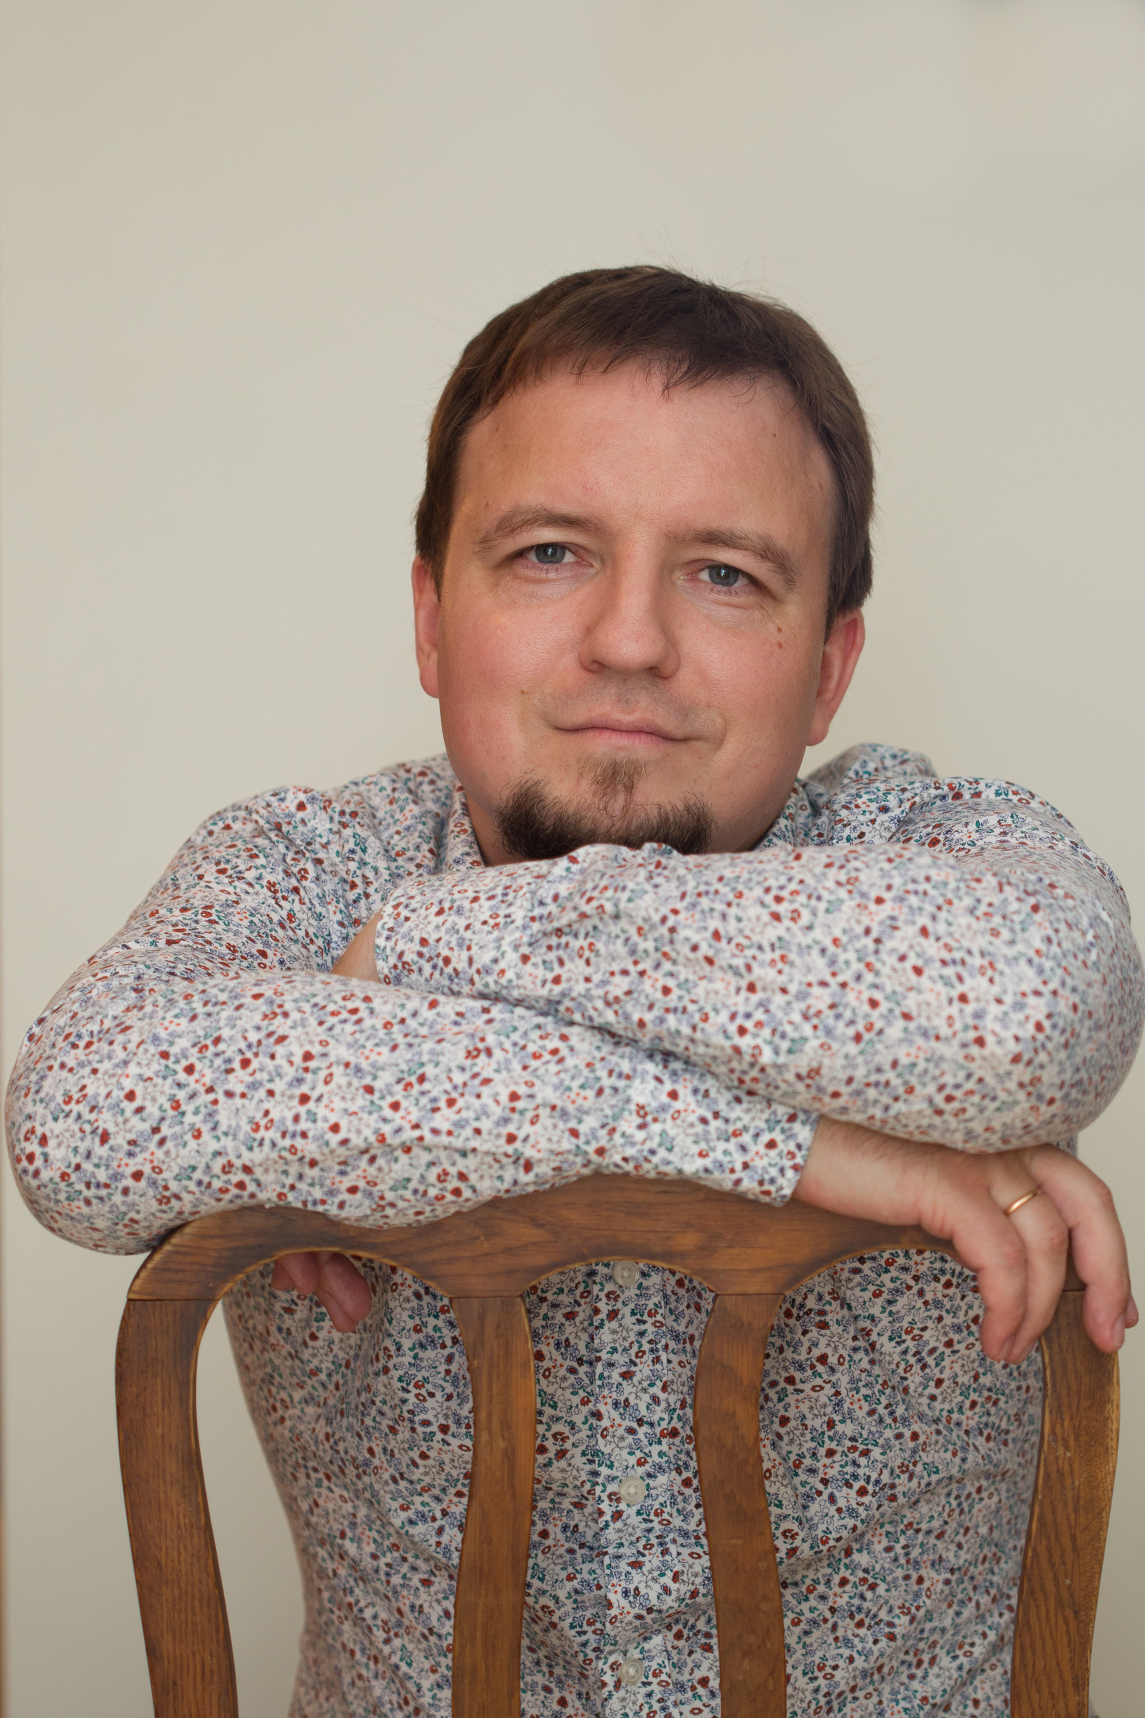
\includegraphics[width=\textwidth]{author.jpg}
		\end{column}
	\end{columns}
\end{frame}

\begin{frame}[fragile]
  \frametitle{How to get a grade}
	\begin{itemize}
	\item Lectures
	\begin{itemize}
		\item Each contact has 6 30-minute blocks
		\item Each block has 
		\begin{itemize}
				\item $\approx$20 minutes of me talking, 
				\item 5 minutes of discussion in pairs on a given topic
				\item 5 minutes of joint discussion
		\end{itemize}
		\item Attending the lectures is not compulsory, attending the final seminar is
	\end{itemize}
	\item \textbf{Group project:} As a group, develop and present an IT strategy 
	\item \textbf{Exam:} Written analytic essay
	\item 70\% of the grade comes from the group project
	\end{itemize}
\end{frame}

\begin{frame}[fragile]
  \frametitle{The Group Project}
  	\begin{itemize}
		\item Group size: $2\leq N\leq6$. \textbf{No exceptions!}
		\note{Start looking for one ASAP. I don't care when you do it or who is in what groups. You don't present, you don't pass \par}
		\item That's how specific the assignment is going to get
		\note{Just like in real life. Think of me as an investor who needs be assured you know what the hell you are doing\par}
		\item The result is to be presented to the class at the end seminar. Names on the slides are the subject of grading
		\item Success criteria: the organisation is plausibly doing better with the strategy than without
		\item Grading criteria: the people present have been assured this is so
	\end{itemize}
\note{That's the most important part of the class. You don't want to rush it.}
\end{frame}

\begin{frame}[fragile]
  \frametitle{Previous experience on group projects}
  	\begin{itemize}
		\item Don't take on too complex tasks: the goal is to mock up the strategy process not solve complex problems
		\note{Or complain later that you colleague took a simple task and got a better grade\par}
		\begin{itemize}
			\item Imaginary organisations are harder than real ones
			\item Public sector is harder than private sector
			\item Big organisations are harder than a small ones
			\note{Beware of trivial man-and-dog companies, though. }
		\end{itemize}
		\item Lean on the structure of the course: all topics we cover in class should be covered in the strategy
		\item Your strategy must be rooted in the business and its strategy
		\begin{itemize}
			\item Don't dictate business strategic choices
			\item Do outline strategic restrictions in place
			\item Don't attempt to fix the company using IT
			\note{If the organisation is not very well run or has a strategy issue, take it for granted\par}
		\end{itemize}
		\item Focus on the presentation. Information you don't deliver does not exist
		\note{Ideally, a few slides of org. background, a slide or two for each topic, a few slides on next steps and a summary}
	\end{itemize}
\end{frame}


\begin{frame}[fragile]
  \frametitle{The exam}
	The exam consists of two short essays discussing topics covered in class
  	\begin{itemize}	
		\item The topics are from among the questions we discuss in class
		\item It is about content, not volume
		\note{I read one A4 per question tops\par}
		\item Experience should work: if the discussion is thorough, it does not matter where it comes from
		\note{But this is tricky as my definition of 'thorough' depends on the discussion in class\par}
		\item The exam gives 30\% of the grade
		\note{Passing the group project means passing the course if you are happy with the grade. Read the syllabus}
	\end{itemize}
\end{frame}

\begin{frame}[fragile]
  \frametitle{Study materials}
	\begin{itemize}
		\item The slides are available
		\item Some blog posts on adjacent topics will be posted about once a week at \url{http://andreskytt.github.io/it_strateegia/}
		\item If somebody wants to contribute to that or disseminate their good quality notes, I'm all ears
		\item \url{https://github.com/andreskytt/it_strateegia}
		\item I'll post the slides and the articles I have copies of to Moodle
		\item The (non-compulsory) bibliography will be included in the slides and posted at the blog
	\end{itemize}
\end{frame}


\begin{frame}[fragile]
  \frametitle{House rules}
	\begin{itemize}
		\item Permitted are 
		\begin{itemize}
			\item Questions including questioning whatever I tell you
			\item Moderate sharing of personal experience
			\item Arrival and leaving whenever
		\end{itemize}
		\item Forbidden is wasting time. Yours and mine
	\end{itemize}
\end{frame}
\note{There's a difference between sharing experience and going way off on a tangent}

\begin{frame}[fragile]
  \frametitle{Structure of the course}
	\begin{itemize}
		\item The structure relies on the IT Manager occupational standard \footnote{\url{http://www.kutsekoda.ee/et/kutseregister/kutsestandardid/10443037}} built on top of EU standards
			\begin{itemize}
				\item Less focus on topics covered in other classes
				\item The goal is to provide a holistic picture including developing relationships between topics
			\end{itemize}
		\item We'll focus on fundamentals
			\begin{itemize}
				\item The strategy is about answering "How do we do things better than others" \citep{de2006strategy}	
				\item To do things better, there must be understanding of \emph{why} we do things in addition to \emph{what} we do
				\item Internal validation: can what I teach be out of fashion in 15 years?
				\item As much personal examples and cases as I can squeeze in and am at liberty of discussing
			\end{itemize}
	\end{itemize}
\end{frame}
\note{ITIL, TOGAF, COBIT, Scrum etc. you can study yourself or pay for dedicated courses. These fashions change. We are at university after all}

\begin{frame}[fragile]
  \frametitle{Course structure}
		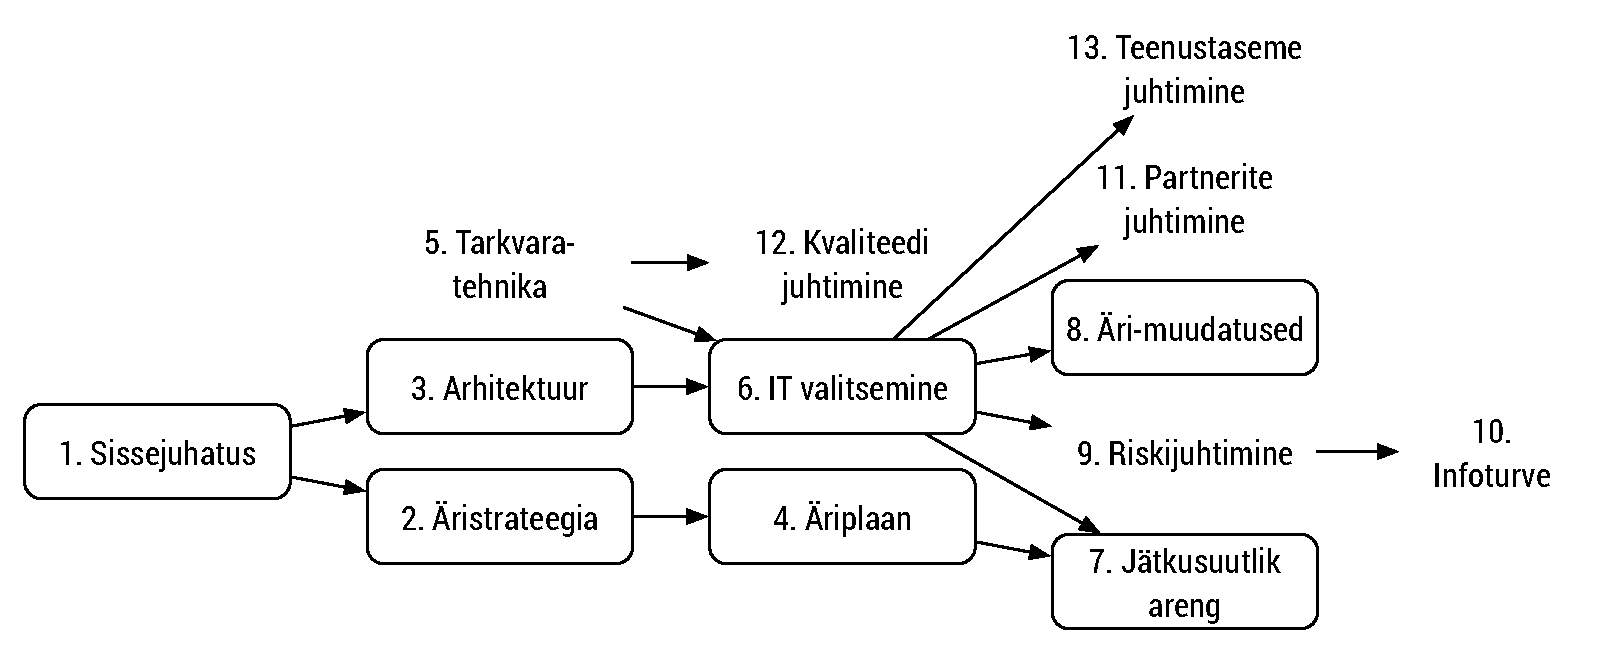
\includegraphics[width=\textwidth]{aine_struktuur.pdf}
\end{frame}
\note{The numbers mean the order of topics covered. In black frames are topics covered in slightly more detail. The arrows indicate logical dependency}

%Arutelu koht
\begin{frame}[fragile]
  \frametitle{Discussion point}
		\begin{center}
			\textbf{What are your expectations towards this course?}
		\end{center}
\end{frame}
		
\section{Business and IT Strategy}

\begin{frame}[fragile]
  \frametitle{On breakfast}
  \begin{quote}
    Culture eats strategy for breakfast
  \end{quote}
	Peter Drucker
	\note{A gentle reminder that if you get culture wrong, none of what we are going to discuss, really matters}
\end{frame}


\begin{frame}[fragile]
  \frametitle{What is strategy?}
  	Strategy is not well defined. Much that is thought of as strategy has little to do with it \citep{de2006strategy, rumelt2011good}. Some themes are fairly common, however:
	\begin{itemize}
		\item Positioning of the organisation for competitive advantage
		\item Choice of markets and economic sectors to participate in
		\item Choice of goods and services offered
		\item Management and dedication of resources
	\end{itemize}
	\textbf{Goal:} Creation of value for owners and other stakeholders via providing value to the customers.
	\note{The meaning of "value" for owners and stakeholders is a non-trivial question}
\end{frame}

%\begin{frame}[fragile]
%  \frametitle{Strategy is dynamic in nature}
%	\vfill
%	\begin{center}
%		Strategy must change at least as fast as it is changing its environment
%		\note{The OODA loop. New environment demands new strategy. We'll discuss this further during our third contact\par}
%	\end{center}
%	\vfill
%\end{frame}


\begin{frame}[fragile]
  \frametitle{The art of war}
  \emph{"Strategos"} - "army leader" in Greek. Sun Tzu "The Art of War" \citep{tzu2013art} is still widely applicable:
  \note{Freedman has criticised this. There are notes in the blog on this}
	The victory has five "essentials". He will win 
   \begin{enumerate}
   		\item who knows when to fight and when not
		\item who knows how to handle both superior and inferior forces
		\item whose army is animated by the same spirit throughout all its ranks
		\item who, prepared himself, waits to take the enemy unprepared
		\item who has military capacity and is not interfered with by the sovereign 
   \end{enumerate}
\end{frame}

\begin{frame}[fragile]
  \frametitle{The art of war}
  \begin{quote}
    All warfare is based on deception
  \end{quote}

\end{frame}

\begin{frame}[fragile]
  \frametitle{Strategy in a wider context}
  Strategy is part of a larger managerial system that, among others, contains at least
  	\begin{description}
		\item[Vision] as a dream of a common bright future
		\item[Mission] as a reason to exist
		\item[Culture] as a set of values enabling coexistance
	\end{description}	
	\begin{quote}
	vision = mission + strategy + culture \end{quote}\citep{lipton1996demystifying}
\end{frame}


\begin{frame}[fragile]
  \frametitle{Dynamics of strategy}
It is clear that
  \begin{itemize}
  	\item There is constant internal and external change not least brought about by execution of the strategy itself
	\note{And these get more and more difficult to predict in the global context\\}
	\item People change
	\note{We all get older and this inevitably shifts our values and outlook on things. Hopefully we get wiser, too\\}
	\item The concept of "value" changes for the owners and stakeholders
	\item Entropy tends to grow as reason requires more energy than randomness
	\note{It is really hard to keep saying 'no'\\}
  \end{itemize}
Therefore strategy is dynamic and
	\begin{itemize}
		\item Gets outdated sooner or later
		\note{The sooner the better it is at changing the world\par}
		\item If not changed, leads to cognitive dissonance within the organisation
		\note{A leader can choose to ignore the reality whereas a front line worker needs to face it\par}
	\end{itemize}
\end{frame}

\begin{frame}[fragile]
  \frametitle{Consequences of the dynamic strategy}
	The process of developing a strategy is as important as the end result
  \note{Eisenhower: Plans are worthless, but planning is everything\\}
	\begin{itemize}
		\item Due to the dynamic nature of strategy, there must be a (hopefully systemic) way to 
		\begin{itemize}
			\item realise we need to change it
			\item ignore it as changes might happen too fast to fall back to it
			\item keep respecting it despite it being constantly challenged and occasionally ignored
		\end{itemize}
		\item Development of a joint direction assumes the ability of an organisation to deal with differences of opinion
		\item It is easier to face a danger shoulder to shoulder. Strategy discussion provides assurance we are still in it together
		\note{That courage might prove more helpful than an actual plan\\}
	\end{itemize}
\end{frame}

\begin{frame}[fragile]
  \frametitle{Strategy as a sequence of decisions}
  Strategy can be seen as a sequence of decisions. What do we do and what do we \emph{don't} do. 
  
  Therefore
	\begin{itemize}
		\item is the process of strategy creation inherently conflicted, just like any decision
		\note{Therefore it is pointless to start working on a strategy without the ability to healthily manage conflict\\}
		\item must strategy provide a recipe for making decisions as not all of them can be foreseen
		\item the strategy document must not be "fluffy"
		\note{Rumlet good strategy/bad strategy}
	\end{itemize}
\end{frame}


%Arutelu koht
\begin{frame}[fragile]
  \frametitle{Discussion point}
		\begin{center}
			\textbf{How to separate the IT strategy from the business strategy?}
		\end{center}
\end{frame}

\begin{frame}[fragile,label={stack}]
	\frametitle{Layered model of the organisation}
	\begin{columns}[t]
		\begin{column}{6cm}
			\begin{itemize}
				\item Every layer is linked to the one below and above it
				\item Illustrates position of technology from an architects perspective
				\item Similar approach to the one found in TOGAF but wider in concept
			\end{itemize}
		\end{column}
		\begin{column}[T]{5cm}
			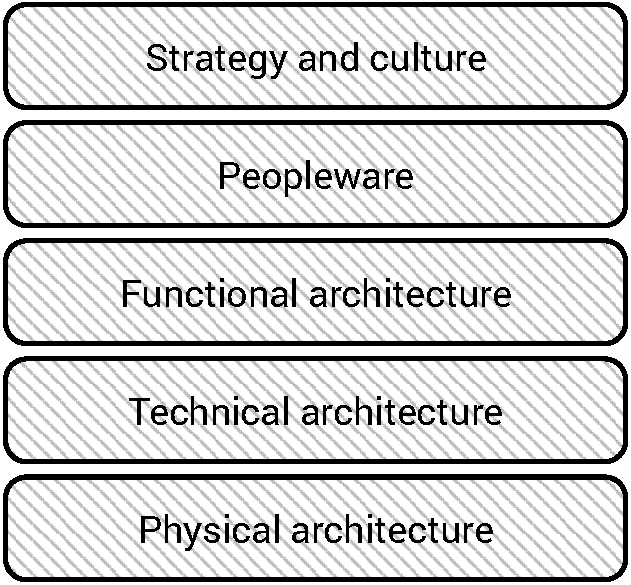
\includegraphics[width=\textwidth]{stack.pdf}
		\end{column}
	\end{columns}
\end{frame}

\begin{frame}[fragile]
  \frametitle{Layers}
  	\begin{description}
		\item[Strategy and culture] Strategic, legal and cultural setup and context of the organisation 
		\item[Peopleware] The structures, processes and systems implementing the strategy 
		\item[Functional architecture] The functional components supporting the processes and structures (e.g. e-mail, ERP, webstore, production line)
		\item[Technical architecture] The concrete technical implementation of the functional architecture 
		\item[Physical architecture] The physical infrastructure everything else is running on including server rooms but also office spaces
	\end{description}
\end{frame}

\begin{frame}[fragile]
  \frametitle{Implications of the model}
  All models are wrong but some models are useful \citep{box1976science}
	\begin{itemize}
		\item All layers are in \emph{constant} change, organisation is (or needs to be) a dynamic construct
		\note{From the dynamic nature of strategy\\}
		\item No change can take place in one layer alone
		\item Isolated changes create "tectonic" tension between layers
		\item Changes propagate down- and upwards with decreasing impact
	\end{itemize}
	Technical and business architectures are commonly the only ones with explicit architecture governance in place
\end{frame}


%Arutelu koht
\begin{frame}[fragile]
  \frametitle{Discussion point}
		\begin{center}
			\textbf{How rapidly do changes abate? Can a change in business strategy cause a change in the hosting architecture?}
		\end{center}
\end{frame}

\begin{frame}[fragile]
  \frametitle{IT-business alignment}
  Various aspects of IT and the organisation are in constant dynamic equilibrium (see \cite{luftman2004assessing})
	\begin{columns}[T]
		\begin{column}{7cm}
			\begin{itemize}
				\item The parties have conflicting interests
				\item It is about balancing interests not winning 
				\item The balance is achieved via organisational structures and processes
			\end{itemize}
		\end{column}
		\begin{column}[T]{5cm}
			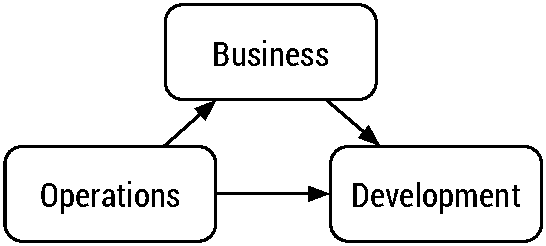
\includegraphics[width=\textwidth]{alignment.pdf}
			\note{Placing all three sides so closely together the balancing becomes unnecessary is the main idea behind devops\\}
		\end{column}
	\end{columns}
\end{frame}

\begin{frame}
	\frametitle{On organisational equilibrium}
	This is a dynamic equilibrium that depends on mutual trust and can deteriorate rapidly
	\begin{itemize}
		\item The Business
		\begin{itemize}
			\item Seeks to maximise "bang-per-buck" at the time horizon they are measured against
			\item They pay the bills, they order the music
		\end{itemize}
		\item The Development
		\begin{itemize}
			\item Love to build complex things regardless of practicality
			\item Dread the mundane (and thus build elaborate tools to avoid it)
		\end{itemize}
		\item The Operations
		\begin{itemize}
			\item Would like to see everything remain exactly as it is now
			\item They know, that they are responsible for everything while controlling nothing
		\end{itemize}
		\note{An architect usually sits smack bang in the middle\\}
	\end{itemize}
\end{frame}

\begin{frame}[fragile]
  \frametitle{Impact of IT via knowledge management}
  The ability to generate, retain and distribute knowledge is a key competitive advantage \citep{david2000diagnosing}. Knowledge management is not doable without information technology
  	\begin{itemize}
		\item On knowledge management and its technical aspects read here: \citep{15.905}
		\begin{itemize}	
			\item we don't understand how knowledge works
			\item it seems to be critical for organisations to be able to function
		\end{itemize}
		\item Therefore: \textbf{do not mess with it!}
		\note{Unless you have a very very good understanding of what you are doing\\}
	\end{itemize}
\end{frame}

\begin{frame}[fragile]
  \frametitle{Impact of IT via process management}
		\begin{center}
			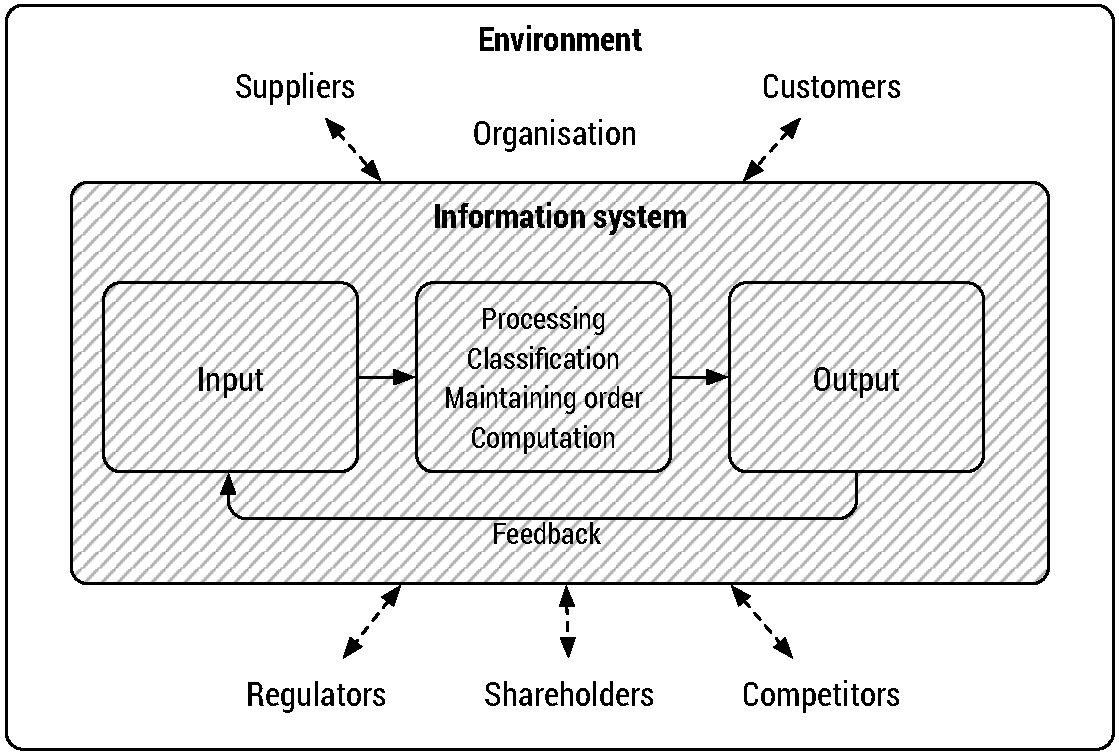
\includegraphics[width=.80\textwidth]{info_org.pdf}\\
		\end{center}
		\cite{laudon2000management}
\end{frame}


%Arutelu koht
\begin{frame}[fragile]
  \frametitle{Discussion point}
		\begin{center}
			\textbf{How to do sensible IT management when the organisation itself is not sensibly managed?}
		\end{center}
\end{frame}

\section{Architecture}

\begin{frame}[fragile]
  \frametitle{Common approach to architecture}
		From the engineers perspective, architecture is a description how things fit together
		\begin{itemize}
			\item Working and proven practice
			\item Good understanding of the strength of a joint does not tell you how to build a good house
		\end{itemize}
		
		From academic perspective, architecture is usually a way to describe something formally and to reach this description
		\begin{itemize}
			\item A lot of work little of which makes it to real life use
			\item Huge amount of incompatible paradigms
			\item Only helps you think about things that can be formalized
		\end{itemize}
		
\end{frame}

\begin{frame}[fragile]
	\frametitle{Vitruvius Pollio}
	\begin{columns}[t]
		\begin{column}{7cm}
			\begin{center}
				\begin{quote}
					\ldots all these must be built with due reference to durability, convenience and beauty
					\note{Vitruvian principles}
				\end{quote}
			\end{center}
			\vskip 1cm
			Marcus Vitruvius Pollio, 80-70 eKr.- 15 pKr  \citep{pollio1914vitruvius}
		\end{column}
		\begin{column}[T]{3cm}
			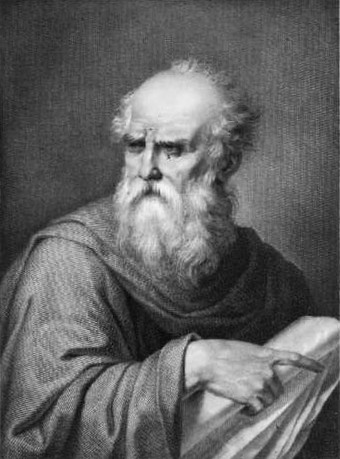
\includegraphics[width=\textwidth]{vitruvio.jpg}
		\end{column}
	\end{columns}
\end{frame}

\begin{frame}[label=Yosemite]
	\frametitle{An example of system boundaries}
	\begin{columns}[t]
		\begin{column}{6.5cm}
			In Q3 2014, Apple fundamentally changed the chip card driver architecture of OS X
			\begin{itemize}
				\item Estonian digital signature software could not be updated in time between announcement and launch
				\item First e-residents joined on 1st of December
				\item A nerve-wrecking mayhem ensued
			\end{itemize}
		\end{column}
		\begin{column}[T]{4.5cm}
			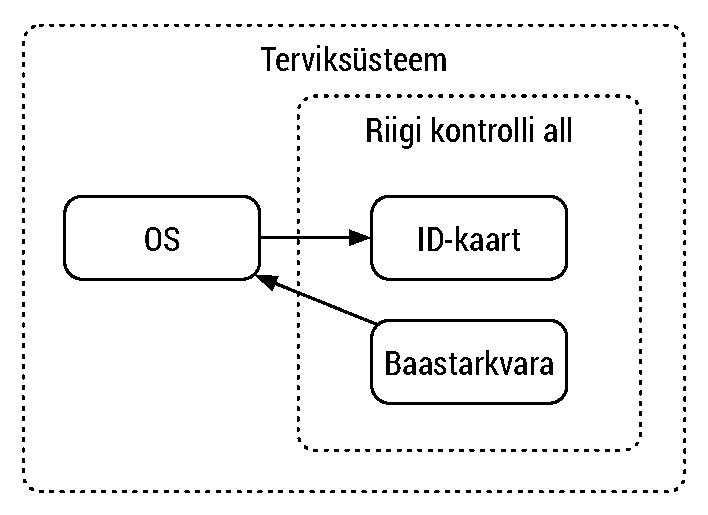
\includegraphics[width=\textwidth]{yosemite.pdf}
		\end{column}
	\end{columns}
\end{frame}


\begin{frame}[fragile]
  \frametitle{On system boundaries}
  		Any declaration of system boundaries is to an extent arbitrary
		\begin{itemize}
			\item Usually this is done based on either control or competences/technology
			\item The system might contain hardware, software and people as well as their relationships
			\item Therefore it is not reasonable to limit discussion of architecture to software
			\note{Well, we already covered organisational architecture a bit}
		\end{itemize}

\end{frame}

\begin{frame}
	\frametitle{More generally on the paradigm shift}
	The following statements hold less and less frequently for organisations
	\begin{enumerate}
		\item Organisations are culturally, technically etc. homogenous		
		\note{You and your architecture can sod off, I know better what works around here (somebody from Montevideost)\\}

		\item Organisational and legal boundaries are well-defined
		\note{Tightly integrated supply chains. Widespread use of coupled platforms. Multinationals ignoring nation-states\\}

		\item Organisations are relatively independent of gloabal problems
		\note{Refugees, climate change, population growth etc. cannot be ignored\\}
		\item The information systems in use have clear tightly controlled boundaries
		\note{Mono-functional hard- and software operated by highly trained professionals vs. multifunctional hard- and software used by random people for random purposes\\}
	
  \end{enumerate}

\end{frame}

\begin{frame}[fragile]
  \frametitle{Definition of a system}
		\begin{center}
  			\begin{quote}
				System is a set of entities the function of which is larger than the sum of the functions of individual ones
			\end{quote}
			\begin{quote}
				System thinking is a way of thinking of a question, circumstance or a problem explicitly as a system
			\end{quote}
		\end{center}
		\cite{crawley2015systems}
\end{frame}



%Arutelu koht
\begin{frame}[fragile]
  \frametitle{Discussion point}
		\begin{center}
			\textbf{What value is added by dealing with architecture?}
		\end{center}
\end{frame}

\begin{frame}
	\frametitle{An alternative approach to architecture}
	An approach rooted in system thinking that overcomes the challenges described previously
	\begin{columns}
		\begin{column}{6.8cm}
			\begin{itemize}
				\item Thinking of systems, we inevitably also think of system architecture
				\item A holistic approach encompassing both functional and technical aspects of a system
				\item Context is taken into account
				\item Well-used in practice, especially in non-software fields
			\end{itemize}
		\end{column}
		\begin{column}{3.2cm}
			\vfill
			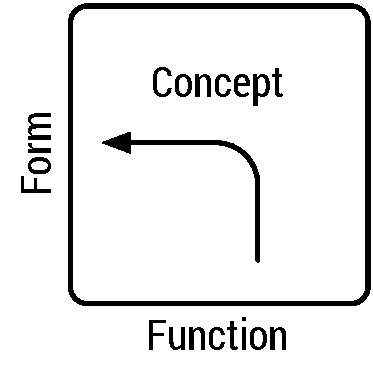
\includegraphics[width=\textwidth]{ffc.pdf}
		\end{column}
	\end{columns}

\end{frame}


\begin{frame}[fragile]
  \frametitle{Architecture is...}
  		\begin{center}
			\begin{quote}
			The embodiment of \textbf{concept}, and the allocation of physical/informational \textbf{function} to elements of \textbf{form}, and definition of \textbf{interfaces} among the elements and with the surrounding \textbf{context}.
			\end{quote}
		\end{center}
	\cite{crawley2015systems} 
\end{frame}

\begin{frame}[fragile]
  \frametitle{Definitions}
	\begin{description}
		\item[Form] That, what \emph{is} + its structure
		\item[Function] That, what is being \emph{done}, mainly structured around a value creation process
		\item[Concept] A \emph{mental model} of a system that links form to function by that embodying the main principles of the system
	\end{description}
\end{frame}
\note{Concept is where organisational culture becomes linked to architecture. This explains why a bank and a startup might solve an identical problem differently}

\begin{frame}[fragile]
  \frametitle{Notes on the model}
	\begin{itemize}
		\item Architecture determines design and operational parameters, design provides their values
		\item Because the model contains structure of things, it is deeply linked with the concept of complexity
		\item Very multidisciplinary approach (engineering, management, leadership, cybernetics, mathematics etc.)
		\item Intrinsically holistic and linked to system thinking
	\end{itemize}
\end{frame}

%Arutelu koht
\begin{frame}[fragile]
  \frametitle{Discussion point}
		\begin{center}
			\textbf{What are the key differences between system architecture and how architecture is commonly seen?}
		\end{center}
\end{frame}

\section{Bibliography}

\begin{frame}[t,allowframebreaks,]
  	\bibliographystyle{plainnat}
	\bibliography{it_strateegia} 

\end{frame}

\section{License}
\begin{frame}{Theme}

  Get the source of this theme and the demo presentation from

  \begin{center}\url{http://github.com/matze/mtheme}\end{center}

  The theme \emph{itself} is licensed under a
  \href{http://creativecommons.org/licenses/by-sa/4.0/}{Creative Commons
  Attribution-ShareAlike 4.0 International License}.

  \begin{center}\ccbysa\end{center}

\end{frame}

\begin{frame}{Content}
	The contents of the slides is lidecensed under a \href{http://creativecommons.org/licenses/by-nc-sa/4.0/}{Creative Commons Attribution-NonCommercial-ShareAlike 4.0 International}
	\begin{center}\ccbyncsa\end{center}
\end{frame}

\plain{Questions?}

\end{document}